%Authors guidlines: http://royalsocietypublishing.org/instructions-authors
% 2500 words max (includes the title page, abstract, references, acknowledgements and figure/table legends)
% current version is around 3700. I think a big cut down can be done on the references.
% We allow a maximum of 4 displays, only 2 of which can be figures.

\documentclass[12pt,letterpaper]{article}


%Packages
\usepackage{pdflscape}
\usepackage{fixltx2e}
\usepackage{textcomp}
\usepackage{fullpage}
\usepackage{float}
\usepackage{latexsym}
\usepackage{url}
\usepackage{epsfig}
\usepackage{graphicx}
\usepackage{amssymb}
\usepackage{amsmath}
\usepackage{bm}
\usepackage{array}
\usepackage[version=3]{mhchem}
\usepackage{ifthen}
\usepackage{caption}
\usepackage{hyperref}
\usepackage{amsthm}
\usepackage{amstext}
\usepackage{enumerate}
\usepackage[osf]{mathpazo}
\usepackage{dcolumn}
\usepackage{lineno}
\usepackage{longtable}
\pagenumbering{arabic}

\newcolumntype{L}[1]{>{\raggedright\let\newline\\\arraybackslash\hspace{0pt}}m{#1}}
\newcolumntype{C}[1]{>{\centering\let\newline\\\arraybackslash\hspace{0pt}}m{#1}}
\newcolumntype{R}[1]{>{\raggedleft\let\newline\\\arraybackslash\hspace{0pt}}m{#1}}

%Pagination style and stuff % NC: Note that these are all syst biol specific.
\linespread{2}
\raggedright
\setlength{\parindent}{0.5in}
\setcounter{secnumdepth}{0} 
\renewcommand{\section}[1]{%
\bigskip
\begin{center}
\begin{Large}
\normalfont\scshape #1
\medskip
\end{Large}
\end{center}}
\renewcommand{\subsection}[1]{%
\bigskip
\begin{center}
\begin{large}
\normalfont\itshape #1
\end{large}
\end{center}}
\renewcommand{\subsubsection}[1]{%
\vspace{2ex}
\noindent
\textit{#1.}---}
\renewcommand{\tableofcontents}{}
%\bibpunct{(}{)}{;}{a}{}{,}

%---------------------------------------------
%
%       START
%
%---------------------------------------------

\begin{document}


\newcommand{\beginsupplement}{%
    \setcounter{table}{0}
    \renewcommand{\thetable}{S\arabic{table}}%
    \setcounter{figure}{0}
    \renewcommand{\thefigure}{S\arabic{figure}}%
}

%Running head
\begin{flushright}
Version dated: \today
\end{flushright}

\bigskip
\medskip
\begin{center}

\noindent{\Large \bf Assessment of cladistic data availability for living mammals}

\bigskip
\noindent{\Large \bf Electronic Supplementary Material 1}

\bigskip
\noindent {\normalsize \sc Thomas Guillerme$^1$$^,$$^*$ and Natalie Cooper$^1$$^,$$^2$}\\
\noindent {\small \it 
$^1$School of Natural Sciences, Trinity College Dublin, Dublin 2, Ireland.\\
$^2$Department of Life Sciences, Natural History Museum, Cromwell Road, London, SW7 5BD, UK.}\\
\medskip
\noindent{*\bf Corresponding author.} \textit{t.guillerme@imperial.ac.uk}\\  
\vspace{1in}

\end{center}
%\modulolinenumbers[1]
%\linenumbers


\newpage


%TG: Maybe useless, I'll add that just in the thesis.
%\section{Graphical abstract}

%\begin{figure}[!htbp]
%\centering
%    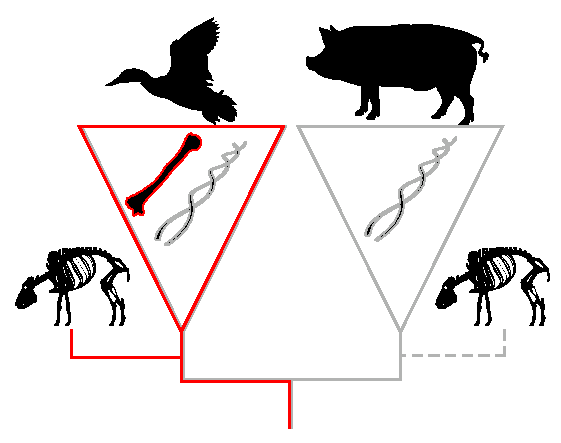
\includegraphics[width=1\textwidth]{MissingDataFigure.pdf}
%\caption{Example of topological errors due to missing morphological data in living taxa.
%The phylogeny contains two clades, Aves and Mammalia, with molecular data (grey) for both but only morphological data (red) for Aves.
%If a mammalian fossil species (with no molecular data) is added to the phylogeny, it will erroneously branch with the Aves instead of the Mammalia because no morphological data will overlap between the fossil mammals and the living ones.}
%\label{Figure_missing_data_problem}
%\end{figure}


\section{1 - Data collection}
\subsection{Public repositories}
We downloaded available matrices containing fossil and/or living mammal taxa from the three data bases using the following list of keywords:

\texttt{Mammalia; Monotremata; Marsupialia; Placentalia; Macroscelidea; Afrosoricida; Tubulidentata; Hyracoidea; Proboscidea; Sirenia; Pilosa; Cingulata; Scandentia; Dermoptera; Primates; Lagomorpha; Rodentia; Erinaceomorpha; Soricomorpha; Cetacea; Artiodactyla; Cetartiodactyla; Chiroptera; Perissodactyla; Pholidota; Carnivora; Didelphimorphia; Paucituberculata; Microbiotheria; Dasyuromorphia; Peramelemorphia; Notoryctemorphia; Diprotodontia}.

Details about each public repository specific search option is listed below.
Note that some matrices have been downloaded from more than one database but that it is not an issue since we are interested in the total number of unique living OTUs and that if some were present in more than one matrix, they still only counted as one single OTU.

\subsubsection{Morphobank}
We accessed the Morphobank repository (\url{morphobank.org}) on the 10th of June 2015 and used the keywords listed above in the search menu.
We downloaded the data associated with each project matching with the keyword.

\subsubsection{Graeme Lloyd}
We accessed Graeme Lloyd's website repository (\url{graemetlloyd.com/matrmamm.html}) on the 10th of June 2015 and downloaded all the matrices that were available with a direct download link in the mammal data section of the website (\texttt{http://graemetlloyd.com/matrmamm.html}).

\subsubsection{Ross Mounce}
We accessed Ross Mounce's GitHub repository (\url{github.com/rossmounce/cladistic-data}) on the 11th of June 2015 and downloaded all 601 matrix.
We then ran a shell script to select only the matrices that had any text element that match with one of the search terms.
% LINK WHICH SHELL SCRIPT
To make the matrix selection more thorough, we ignored the keywords case as well as the latin suffix (\textit{ia}, \textit{ata}, \textit{ea}, and \textit{a}).

\subsection{Google scholars (accessed 11th of June 2015)}
To make sure we didn't miss any extra matrix that wasn't available on one of these repositories, we ran a Google Scholar search on the 5th of January. 
We downloaded the additional cladistic matrices from the 20 first search results matching with our selected keywords and with any of the 35 taxonomic levels (mammals Orders, Infraclasses and Class).
We used the following key words:

\texttt{\textit{order} ("morphology" OR "morphological" OR "cladistic") AND characters matrix paleontology phylogeny}

were \textit{order} was replaced by all the keywords listed above. For each 33 keywords, we selected the 20 first papers to match the Google search published since 2010 resulting in 660 papers.
Among these papers, not all contained relevant data (discrete morphological characters AND mammalian data).
We selected only the 20 first results per search term to avoid downloading articles that were too irrelevant. Among the 660 papers, only 50 contained a total of 425 extra living OTUs (Figure ~\ref{Supp_figure_google_searches}).
Also we decided to select only the articles published since 2010 because nearly every one of the recent published matrix contains both a fraction of morphological characters and OTUs from previous studies.
For example in primates the character \textit{p7} coded first by \cite{ross1998phylogenetic} is reused with the same living species in \cite{seiffert2003fossil}, \cite{marivaux2005anthropoid}, \cite{seiffert2005basal}, \cite{bloch2007new}, \cite{bloch2007new}, \cite{kay2008anatomy}, \cite{silcox2008biogeographic}, \cite{seiffert2009convergent}, \cite{tabuce2009anthropoid}, \cite{boyer2010astragalar}, \cite{seiffert2010fossil}, \cite{marivaux2013djebelemur} and \cite{ni2013oldest}.

\begin{figure}[!htbp]
\centering
    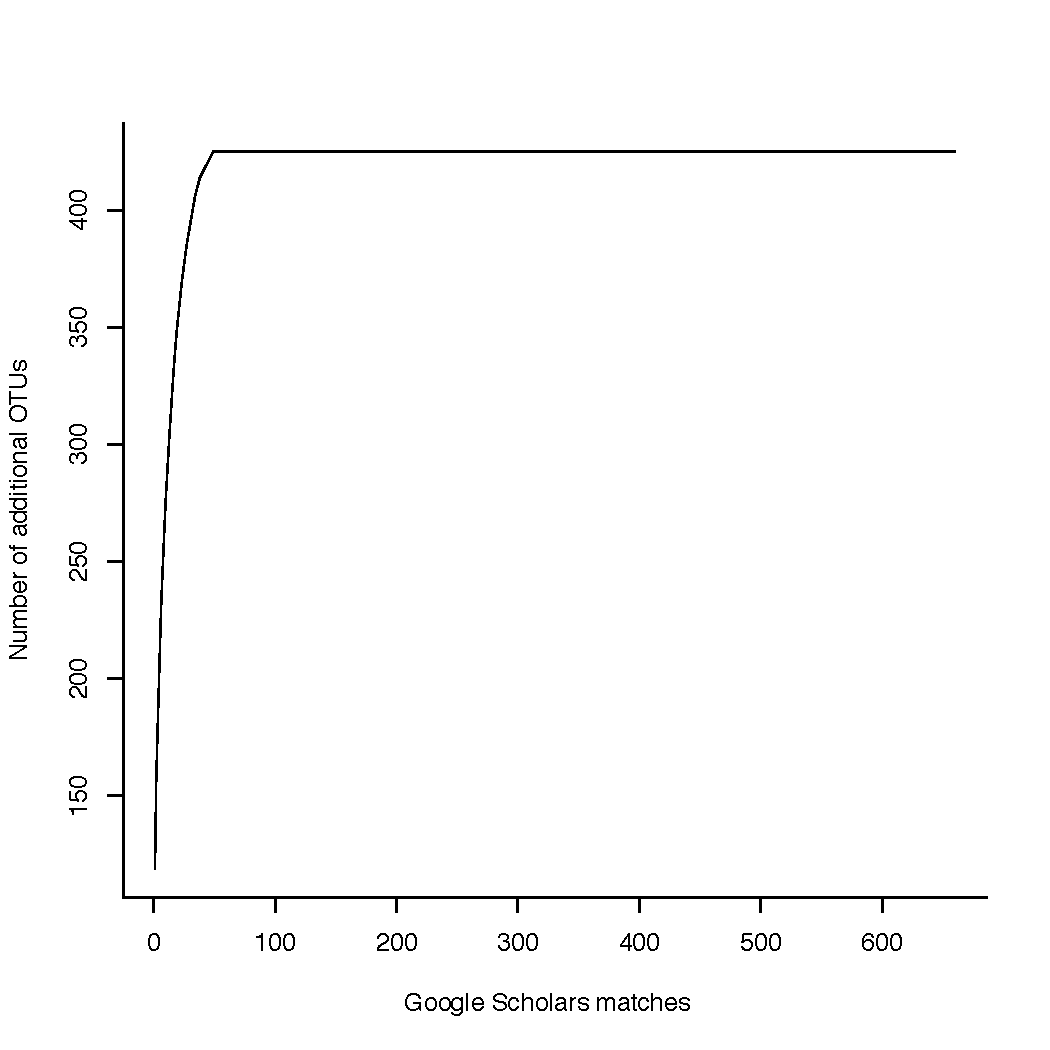
\includegraphics[width=1\textwidth]{Supp_figure_google_searches.pdf}
\caption{Google searches additional OTUs rarefaction curve. The x-axis represent the number of Google Scholar matches (papers, books or abstracts) and the y-axis represents the cumulative number of additional living OTUs per google scholar match.}
\label{Supp_figure_google_searches}
\end{figure}

The list of all the 286 download matrices is available on \url{github.com/TGuillerme/Missing_living_mammals/tree/master/Data/Matrices}.
The matrices contained a total of 11010 operational taxonomic units (OTUs) of which 5228 were unique.
In this study, we refer to OTUs rather than species because the entries in the downloaded matrices were not standardised and ranged from specific individual specimen names (i.e. the name of a collection item) to the family-level.
Where possible, we considered OTUs at their lowest valid taxonomic level (i.e. species) but some OTUs were only valid at a higher taxonomic level (e.g. genus or family).
Therefore for some orders, we sampled more genera than species.

\subsection{Standardising the matrices}
We transformed all the non-nexus matrices (tnt, word, excel, jpeg) to nexus format manually.
We then cleaned the nexus matrices by removing any extra information (trees, continuous characters, morphological characters description, molecular data) to end up with nexus matrices containing only the discrete morphological data.
We then manually fixed the incorrectly-formatted binomial names (e.g. \textit{H. sapiens} became \textit{Homo sapiens}) using the abbreviation list in the concerned publications. 
All the standardised matrices are available on \url{github.com/TGuillerme/Missing_living_mammals/tree/master/Data/Matrices_binomial/Matrices}.

\subsection{Selecting the living OTUs}
%To select the lowest valid taxonomic level for each OTU, we standardised their taxonomy by correcting species names so they matched standard taxonomic nomenclature (e.g., \textit{H. sapiens} was transformed to \textit{Homo sapiens}).
We designated as ``living'' all OTUs that were either present in the phylogeny of \cite{bininda-emondsthe2007} or the taxonomy of \cite{wilson2005mammal}, and designated as ``fossil'' all OTUs that were present in the Paleobiology database (\url{https://paleobiodb.org/}).
For OTUs that did not appear in these three sources, we first decomposed the name (i.e. \textit{Homo sapiens} became \textit{Homo} and \textit{sapiens}) and tried to match the first element with a higher taxonomic level (family, genus etc.).
Any OTUs that still had no matches in the sources above were designated as non-applicable (NA; Figure ~\ref{Supp_figure_Taxonomic_algorithm}).

\begin{figure}[!htbp]
\centering
    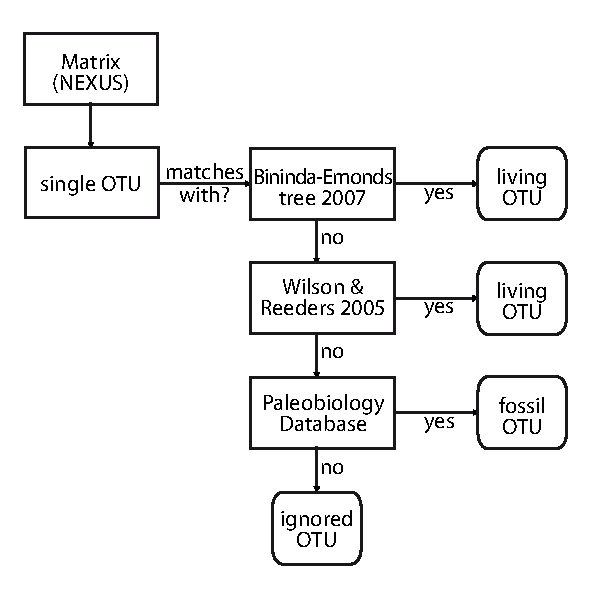
\includegraphics[width=1\textwidth]{Supp_figure_Taxonomic_algorithm.pdf}
\caption{Taxonomic matching algorithm used in this study. For each matrix, each operational taxonomic units (OTU) is matched with the super tree from Fritz 2009. If the OTU matches, then it is classified as living. Else it is matched with the Wilson \& Reeders 2005 taxonomy list. If the OTU matches, then it is classified as living. Else it is matched with the Paleo Database list of mammals. If the OTU matches, then it is classified as fossil. Else it is ignored.}
\label{Supp_figure_Taxonomic_algorithm}
\end{figure}

\section{2 - Data reproducibility}
Every step of the analysis (apart from downloading and standardisation of the matrices) is entirely repeatable via GitHub (\url{github.com/TGuillerme/Missing_living_mammals}).
%Needs to fix this in GitHub
%1-Rarefaction ?
%2-Selecting the OTUs
%3-Analysing the availability and the data structure

\bibliographystyle{vancouver}
\bibliography{Supp_References}

\end{document}